\subsection{Development Process}
The minimum viable artefact is a Python notebook file contains Python scripts to run the experiment.

As discussed in the Research Design section, we configure the ansatz objects such that their gradient variances decrease exponentially with the number of qubits.
These characteristics are:
\begin{itemize}
    \item The circuit depth;
    \item The amount of qubits to be measured for the cost function;
    \item The randomized parameters.
\end{itemize}

\subsubsection{Creating Ansatzes}
We have chosen two ansates \textit{NLocal} and \textit{TwoLocal} from Qiskit circuit library due to their widely used in quantum machine learning.
An example of circuits generated by Qiskit is visulised in Figure \ref{Ansatz samples}.

\begin{figure}
    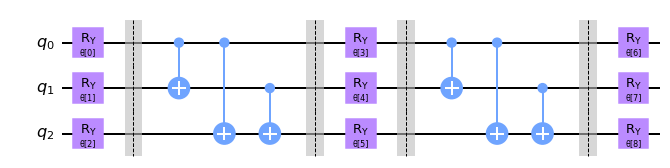
\includegraphics[width=\textwidth]{Artefact/Appendices/ansatz3-2.png}
    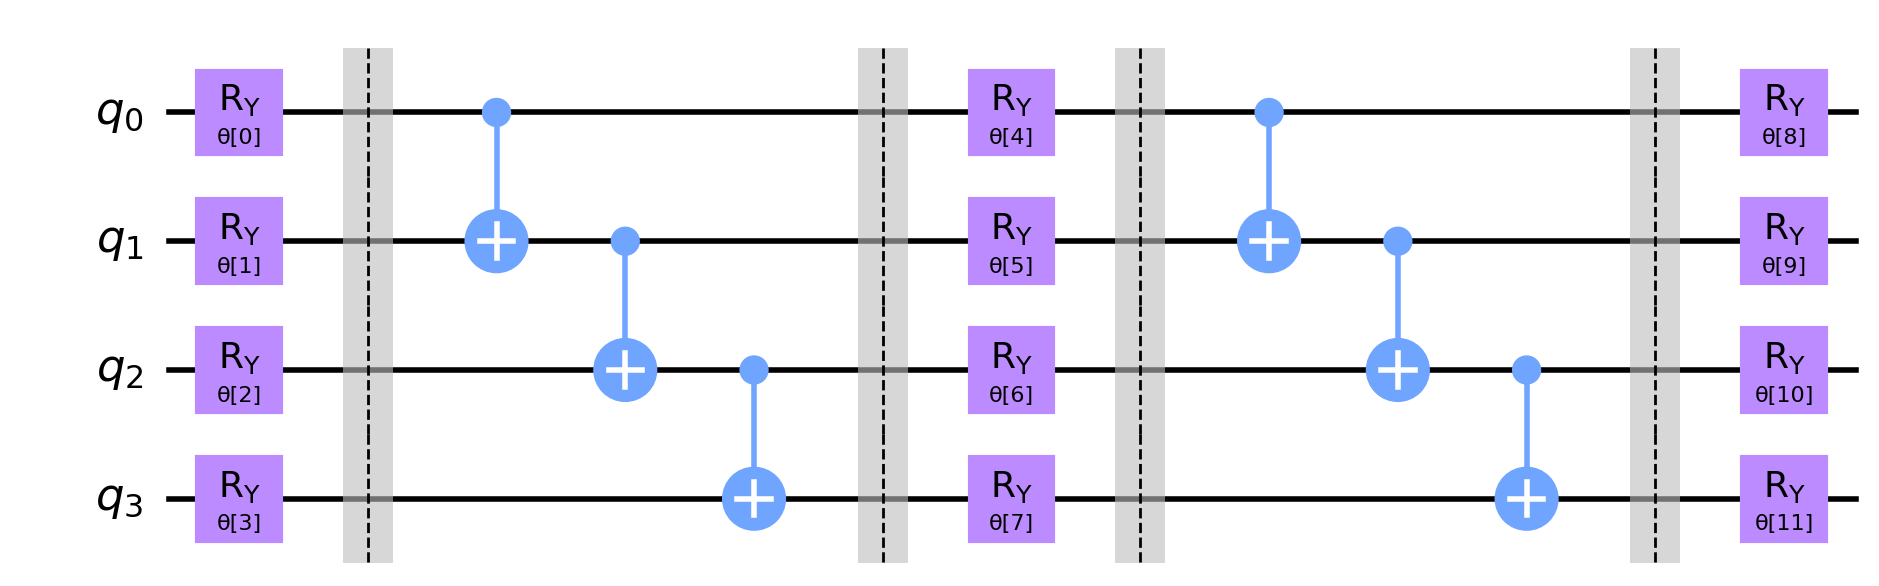
\includegraphics[width=\textwidth]{Artefact/Appendices/ansatz4-2.png}
    \caption{
        Samples of parameterized circuit generated by Qiskit framework.
        The ansatz is a sequence of roration layers and entanglement layers.
        Above: an ansatz of three qubits and two repetition layers.
        Below: an ansatz of four qubits and two reprtition layers.
    }
    \label{Ansatz samples}
\end{figure}

\subsubsection{Visualize the Vanishing Gradient}
To calculate the variance of the gradient, we use the parameter shift rule to yields different sampling value from the ansatz.
The BP phenomena can be verified when the variance of the gradient with increased number of qubits and repetition layers.

For each ansatzes, we have chosen a range of random parameters as the initial starting point.
Such parameters are generated 100 times uniformly randomized to calculate the variance from the ansatz gradient.
We then plot the variance values of the gradients for different number of qubits and repetition value, for a range of 2 to 9 qubits and repetition.

\subsubsection{Experiment with Local Cost Function and Shallow Depth}
The two ansatzes are configured such that their depths are fixed, along with a local cost function.
The \textit{Global Cost Function} is the combined output of all qubits, on the other hand, the \textit{Local Cost Function} only compares the values of individual qubits or a subset of qubits \cite{cerezoCostFunctionDependent2021}.